\chapter{Käytännön esimerkki\label{example}}

Tutkielmassa on nyt käsitelty DevOps-toimintamallia ja sen yhteydessä käytettäviä julkaisutapoja ja orkestrointiratkaisuja.
Osana tutkielmaa esitetään käytännön esimerkki käsiteltyjen aiheiden käytöstä ohjelmistotuotannossa.
Helsingin Yliopiston Norppa-palautejärjestelmän kehitys perustuu DevOps-toimintamalliin ja palvelu käyttää monia tutkielmassa käsiteltyjä teknologioita.
Palvelun perustoiminta ja ohjelmistoarkitehtuuri esitetään tässä luvussa.

\section{Norppa-palautejäjestelmä}

Helsingin yliopiston tietojenkäsittelytieteen osaston sovelluskehitysakatemian (\textit{Toska}) \cite{Tenhunen23} kehittämä kurssipalautejärjestelmä Norppa on tutkielmassa esitetyn DevOps-toimintamallin mukaisessa aktiivisessa kehityksessä.
Järjestelmää käytetään Helsingin Yliopiston lisäksi myös Tampereen yliopiston kurssipalautejärjestelmänä \cite{Tampere23}.

Norppa on integroitu Sisu-opintotietojärjestelmän kanssa.
Järjestelmä luo automaattisesti muokattavan palautelomakkeen ja tiedottaa Sisussa luodun kurssin opiskelijoille palautteen aukeamisesta.
Annetusta palautteesta luodaan yhteenveto, joka näytetään kurssin opiskelijoille ja opettajille.
Norppa tukee myös muun muassa avointa tekstuaalista jatkuvaa palautetta ja koulutusohjelma- sekä yliopistotason palautteen yhteenvetonäkymiä.

Järjestelmän on kehittänyt Helsingin Yliopiston Toska-tiimi, mutta jatkokehitystä tehdään yhteistyössä Tampereen yliopiston kanssa.
Kehitys perustuu avoimeen lähdekoodin ja DevOps-toimintamalliin.
Seuraavaksi esitellään Norpan kehityksessä ja tuotantokäytössä käytetyt tutkielman kannalta merkitykselliset ratkaisut.

\section{DevOps-toimintamallin käyttö}

Norppa on avoimen lähdekoodin projekti, jonka lähdekoodi ja versiohistoria säilötään GitHub-alustalla.
DevOps-toimintamallin mukainen jatkuva integraatio ja toimitus toteutetaan osana versiohallintaa \textit{GitHub Actions}-palvelun avulla.
Kaikissa toimintamallin vaiheissa käytetään konttiteknologiaa ja orkestrointiratkaisuna toimii Kubernetekseen perustuva OpenShift-konttiorkestraatioalusta.

Kuva \ref{fig:norppa:deployment} esittää Norpan julkaisuputken ja käytetyt analytiikkapalvelut.
Kehittäjän viedessä uuden koodimuutoksen versiohallintaan uudesta koodiversiosta rakennetaan automaattisesti kontti, jota vasten suoritetaan testit.
Testauksen onnistuessa sama kontti viedään \textit{Quay.io}-konttirekisteriin, josta se haetaan julkaistavaksi testiympäristöön.
Uuden koodimuutoksen vieminen tuotantoympäristöön vaatii manuaalisen hyväksynnän, jonka seurauksena sama prosessi toistetaan, mutta julkaistu kontti merkitään vietäväksi tuotantoympäristöön.

\begin{figure}[ht]
\begin{center}
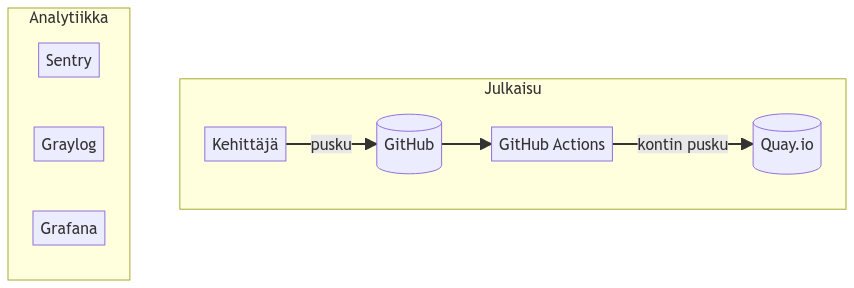
\includegraphics[width=1\textwidth]{figures/norppa_deployment.png}
\caption{Norpan julkaisuputki ja analytiikkapalvelut \cite{Norppa23}\label{fig:norppa:deployment}.}
\end{center}
\end{figure}

Koko julkaisuputki kestää noin viisitoista minuuttia ja mahdollistaa näin useat päivittäiset julkaisut.
Uusia toiminnallisuuksia tuodaan käyttöön osittain pienten yksittäisten julkaisujen kautta, jonka seurauksena koodimuutoksista saadaan nopeaa palautetta ja mahdollisiin ongelmiin voidaan reagoida nopeasti.

\section{Konttien orkestroinnin käyttö}

Norpan testi- ja tuotantoympäristönä toimii yliopiston OpenShift-konttiorkestraatioalusta.
OpenShift on Kubernetekseen perustuva konttiorkestraatioalusta, joka tarjoaa konttien orkestroinnin lisäksi muun muassa käyttäjähallinnan ja oman graaffisen käyttöliittymänsä \cite{Lossent17}.
Kuvassa \ref{fig:norppa:deployment} esitetty julkaisuputki ja erillisellä virtuaalikoneella toimivat analytiikkapalvelut sijaitsevat OpenShift-klusterin ulkopuolella.

Kuva \ref{fig:norppa:architecture} esittää Norpan ohjelmistoarkkitehtuurin osana OpenShift-klusteria.
Norppa koostuu ydinpalvelusta ja siihen liitettävistä erillisistä mikropalveluista.
Tämä arkkitehtuuriratkaisu mahdollistaa palvelun muokattavuuden.
Helsingin ja Tampereen yliopistot käyttävät samaa Norpan ydintä, mutta muut palvelut on toteutettu erikseen yliopistojen tarpeiden mukaisesti.

\begin{figure}[ht]
\begin{center}
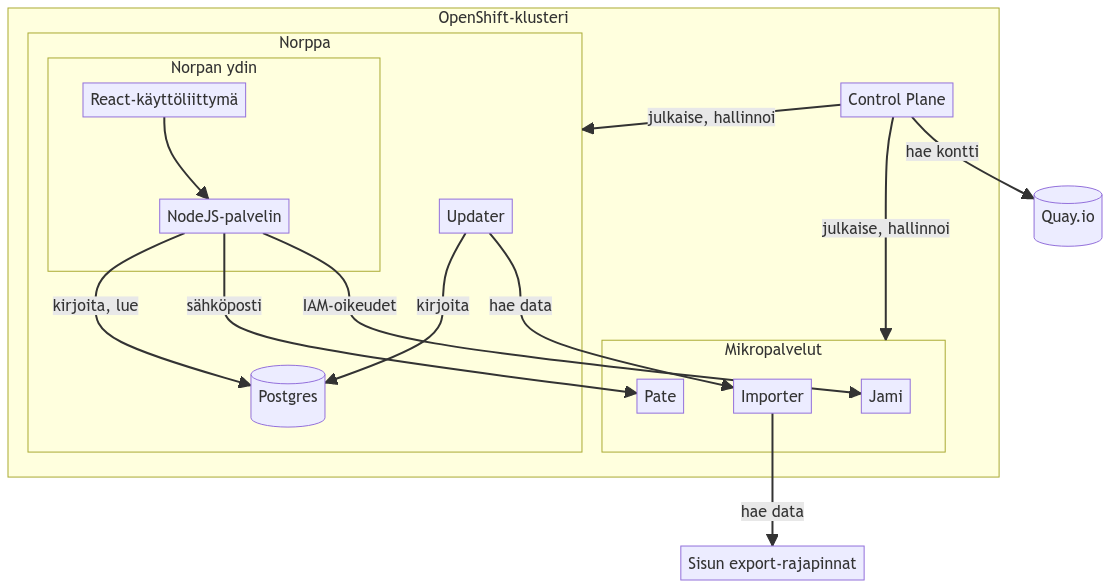
\includegraphics[width=1\textwidth]{figures/norppa_architecture.png}
\caption{Norpan laajennettu arkkitehtuuridiagrammi \cite{Norppa23}\label{fig:norppa:architecture}.}
\end{center}
\end{figure}

Norpan ydin muodostuu React pohjaisesta käyttöliittymästä ja NodeJS-palvelimesta.
Sisusta haetun opintodatan synkronisoinnista huolehtii erillinen Updater-palvelu.
Tämän lisäksi Norppa käyttää useita myös muiden järjestelmien käyttämiä mikropalveluita, kuten sähköpostipalvelua Pate ja käyttöoikeushallintapalvelua Jami.

Kaikki palvelut sijaitsevat samassa OpenShift-klusterissa, joka mahdollistaa helpon palveluiden välisen kommunikaation.
OpenShift-klusteri hakee \textit{Quay.io}-konttirekisteristä uuden kontin julkaisun yhteydessä ja huolehtii käytössä olevien konttien päivityksestä.
Julkaisujen lisäksi klusteri huolehtii luvun \ref{platforms} mukaisesti muun muassa resurssien käyttörajojen hallinnasta ja automaattisesta skaalautumisesta.
